\chapter{}{{Multi-Model Approach to Solar Irradiance Forecasting}}{Multi-Model Blending Approach to Solar Irradiance Forecasting}

\subchapter{Overview}
\par Downward shortwave radiation flux, synonymous with global horizontal irradiance (GHI) is measured by NWP models using columnar radiative transfer models (RTM). The RTMs help in determining cloud optical properties for different wavelength bands with the help of weather variables such as air temperature, gas concentrations and cloud structure. These cloud properties are essential for effective cloud modeling as they determine the absorption, scattering and reflection of global solar radiation. Thus, they contribute to effective shortwave radiation flux computation. However, the direct output from the mesoscale models has shown severe deviations between forecasted and real irradiance \cite{multimodel_ghi}. 

\par While the usage of additional weather variables in machine learning models have shown to improve the post-processing of NWP models by incorporating site-specific information, it has to be taken into consideration that there is a significant variability in the GHI measured by the NWP models with respect to the cloud conditions. Mathiesan et al \cite{multimodel_overpredict} found that the NAM Forecast model tends to overpredict GHI in clear-sky conditions, i.e. conditions in which visible clouds are absent, by up to 40 percent. Thus, effectively identifying the clear-sky conditions becomes essential, following which the bias in GHI measured by the NAM Forecast System in these conditions can be corrected.

\par There are multiple empirical solar radiation formulations which have been extensively discussed in literature \cite{litrev_pvlib10}\cite{litrev_pvlib11}\cite{litrev_pvlib12}\cite{litrev_pvlib13}\cite{litrev_pvlib14}\cite{litrev_pvlib9}, which compute the irradiance metrics from environmental conditions such as cloud cover. These can be broadly classified into decomposition models and parametric models. Using assumptions on solar geometry and transmittance, the former are used to estimate direct beam and diffuse irradiance. The latter are useful for approximating daily solar radiation reaching tilted surfaces. GHI can be empirically estimated from these irradiance metrics. In this \restoregeometry\noindent section, two such empirical solar radiation models, \textit{Clear-Sky Scaling} and \textit{Liu-Jordan Model} are discussed, which help estimate GHI, DHI and DNI. Using measures such as clear-sky index which is useful to separate clear-sky conditions from cloudy conditions; and clearness index, which is the measure of clearness of the atmosphere, GHI measured by NAM Forecast System can be empirically corrected in conditions where visible clouds are absent.

\subchapter{Empirical Solar Radiation Models}
\par Solar researchers have developed various empirical formulations which help in determining the relation between different components of solar radiation and various meteorological parameters. These can be broadly classified into \textit{decomposition} and \textit{parametric} models. The parametric models require information about atmospheric conditions such as turbidity, cloud cover, etc. to be able to formulate the different components of solar irradiance such as diffuse horizontal irradiance (DHI), direct normal irradiance (DNI) and global horizontal irradiance (GHI). Decomposition models formulate equations to estimate the solar irradiance components based on the corerlations between them. Such formulations are relevant, especially in cases where meteorological data is not adequately available.

\par DHI is the amount of solar radiation received by a horizontal surface, which has been scattered by the molecules and particles in the atmosphere. It is the part of the solar radiation which does not belong to the $5^{\circ}$ field of view concentric around the sun, and is typically measured with a pyranometer. DNI is the direct radiation received on a plane normal to the sun over the total solar spectrum. It is an essential component of global irradiance, especially in cloudless conditions, and can be measured with the help of a pyrheliometer. While the solar radiation incident on the earth's atmosphere is relatively constant, various factors such as atmospheric conditions, latitude of the location, season of the year, etc. affect the amount of solar radiation incident on the earth's surface. GHI is the total amount of such terrestrial irradiance which is received by a surface horizontal to the surface of the earth. It can measured with the help of pyranometers, and in general, can be computed from DHI and DNI using the following equation, where $\theta_z$ is the \textit{zenith angle} (the angle between sun and the vertical):
\begin{equation}\label{eq:ghi}
    GHI = DHI + DNI . cos(\theta_z)
\end{equation}

\par Holmgrem et al \cite{pvlib_Holmgren2018} contributed to building \textit{pvlib-python}\footnote{\url{https://github.com/pvlib/pvlib-python}} an open source, python-based tool, ported from the PVLIB MATLAB toolbox developed at Sandia National Laboratories. This software provides a set of utilities for simulating the performance of the photovoltaic energy systems, with implementations of algorithms related to solar energy. Specifically, it contains components to obtain weather forecast data from NOAA/NCEP/NWS models including the GFS, NAM, RAP, HRRR, and the NDFD, retrieved from the UNIDATA THREDDS servers; and components to convert this weather forecast data into a PV power forecast. 

\par For our experiments, we created a NAM weather forecast dataset for the years of 2017 and 2018, retrieved from the NCEP servers. Meanwhile, \textit{pvlib-python} retrieves NAM CONUS 12km resolution forecasts from the THREDDS servers. The key difference between each of these NAM products is that the former is a full complement of both the pressure level fields and surface-based fields, while the latter is a full complement of just the surface-based fields. The NAM data retrieved and processed by \textit{pvlib-python} consists of the following parameters: air temperature, wind speed, total clouds, low clouds, mid clouds and high clouds. In order to be able to use the \textit{pvlib-python} functionalities on the weather forecast dataset collected by us, equivalent surface-level fields were identified in our weather forecast dataset. Thus, compatibility between the NAM data obtained from both the sources was established, enabling the use of \textit{pvlib-python} functionalities on this engineered dataset.

\par \textit{pvlib-python} software contains components, which are implementations of several theoretical formulations to compute irradiance metrics such as DHI, DNI and GHI from the weather forecast data. In this work, each of these irradiance metrics were computed from the \textit{pvlib-python} compatible NAM dataset using two empirical techniques implemented in the software: Clearsky Scaling, Liu-Jordan Model.

\subsubchapter{Clear-sky Scaling}
\par Global horizontal irradiance can be measured with the help of a pyranometer on a horizontal surface, and thus, is typically the most common type of irradiance measurement. Knowledge of the clear sky conditions (absence of visible clouds), is a key requirement for forecasting all three irradiance metrics. Clear-sky models estimate the terrestrial solar radiation under a cloudless sky from various atmospheric conditions. Such models can be generally validated by comparing the measured irradiance in the clear-sky conditions. 

\par Several parametric models have been proposed in literature to compute these irradiance metrics from environmental conditions such as atmospheric turbidity, fractional sunshine, perceptible water vapor, etc. Ineichen et al \cite{pvlib_ineichen} formulated a model to compute Linke turbidity independent of the airmass, and clear-sky GHI from this metric. Going by Larson et al's \cite{pvlib_larson} work, \textit{pvlib-python} scales global horizontal irradiance on the basis of the total cloud cover and clear-sky GHI according to the following equation, where $GHI_{CS}$ is the clear-sky GHI and TCC is the total cloud cover:
\begin{equation}\label{eq:ghi_cs}
    GHI = GHI_{CS} . [0.35 + 0.65(1 - TCC)]
\end{equation}

\par Maxwell et al \cite{pvlib_disc} introduced the popular \textit{Direct Insolation Simulation Code} (DISC) model to compute cloudy-sky DNI from GHI (in this case, computed with Eq. \ref{eq:ghi_cs}) and other environmental factors. Clearness index is the fraction of the solar radiation transmitted through the atmosphere to strike the earth's surface. DISC model uses empirical relationships between the direct and global components of this measure to estimate the direct beam component. Additionally, the clear-sky DHI component can be evaluated from these irradiance metrics and the solar zenith angle using the equation described in Eq. \ref{eq:ghi}.

\subsubchapter{Liu-Jordan Model}
Decomposition models typically utilize only data pertaining to global radiation to estimate diffuse radiation from global solar irradiation data, as can be seen in the previous subsection. They are based on the atmospheric effects in an isolated place, varying according to time of the year, season and climatic conditions \cite{pvlib_liujordan}. Liu et al proposed one of the earliest and simplest models of radiation, the Liu-Jordan model \cite{pvlib_liujordan2}, which presumes that diffuse radiation intensity is distributed uniformly over the whole sky, and helps estimate diffuse radiation on inclined surfaces. In this model, the diffuse irradiance on a surface tilted towards the equator at an angle $\theta$, where $I_D$ is the diffuse radiation on a horizontal surface is given by the following empirical equation:
\begin{equation}\label{eq:lj_dhi}
    I_{Dt} = I_D . (\frac{1 + cos\theta}{2})
\end{equation}

Liu-Jordan model, though simple, is one of the more accurate among isotropic models for estimating diffuse radiation on inclined surfaces \cite{pvlib_liujordan3}. This model helps determine direct normal irradiance, global horizontal irradiance from properties such as extraterrestrial flux, transmittance, and optical air mass number. It has been observed that the Liu-Jordan model provides a good fit to empirical data under overcast skies, but underestimates the solar radiation on tilted surfaces when used for partially-clear and clear-sky days \cite{pvlib_liujordan4}.

\subchapter{Experiment Setup}
\par In this chapter, three series of experiments are performed towards predicting solar irradiance on each of the solar arrays A, B and E. Firstly, solar irradiance forecasting using Numerical Weather Prediction (NWP) models such as North America Mesoscale (NAM) Forecast Model is investigated, replicating the modeling methodology employed in \cite{thesis_zach}. This is compared with the processed NAM dataset obtained, by incorporating the input selection technique described in 3.2. Secondly, a multi-model blending approach is explored, combining the irradiance metrics from NAM Forecast Model and formulations such as Clear-Sky Scaling and Liu-Jordan model in PVLIB. Thirdly, the effect of the spatial expansion of forecast coverage is investigated, by including the weather parameters from a grid of cells around the grid representing Athens. Each of these methodologies are explained in finer detail.

\par Downward shortwave radiation flux (synonymous with global horizontal irradiance, GHI) was identified to be the most important NAM Weather Forecast Model parameter for solar irradiance forecasting. However, a need to correct the bias in the estimation of this parameter was identified. Irradiance metrics such as global horizontal irradiance (GHI), direct normal irradiance (DNI) and diffuse horizontal irradiance (DHI) can be estimated with the help of several formulations defined in literature. With the help of implementations of empirical solar radiation models such as Clear-Sky Scaling and Liu-Jordan model in \textit{pvlib python}, these metrics were estimated from the weather parameters in the NAM data.

\begin{figure}[ht]
    \begin{center}
    	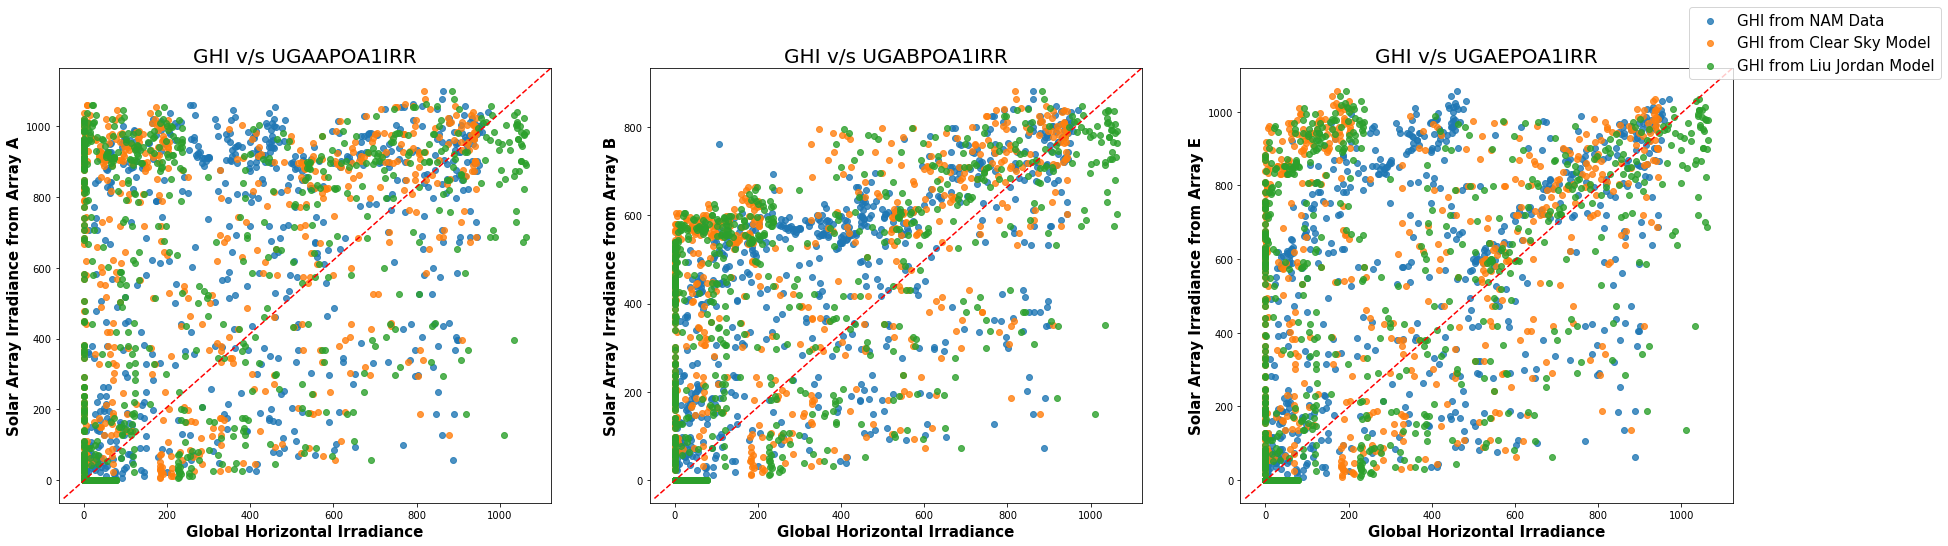
\includegraphics[width=\textwidth]{chapter4/fig_ghi_irradiance.png}
    	\caption[Global horizontal irradiance from NAM data, Clear-sky Scaling and Liu-Jordan against irradiance observations from arrays A, B and E through 2017.]{Global horizontal irradiance from NAM data, Clear-sky Scaling and Liu-Jordan Model against irradiance observations from dual-axis array A (left), fixed-axis array B (center) and single-axis array E (right) through 2017.}
    	\label{fig:fig_ghi_irradiance}
    \end{center}
\end{figure}

\par In this section, a multi-model blending approach is explored, where the weather forecast parameters from NAM are integrated with the irradiance metrics retrieved from Clear-Sky Scaling technique and Liu-Jordan model. Primarily, techniques are explored to combine the GHI parameter from each of the models based on measures such as \textit{clear-sky index} and \textit{clearness index} which are described in greater detail in the following sections. In Fig. \ref{fig:fig_ghi_irradiance}, the GHI parameter estimations from each of the models are plotted against the solar irradiance observations from the dual-axis tracking solar array (array A), fixed-axis solar array (array B) and single-axis solar array (array E) in the solar farm. 

\subsubchapter{Blending NAM Forecast Model and Clear-Sky Scaling Technique}
The clear-sky scaling technique in \textit{pvlib-python} helps estimate the global horizontal irradiance in clear-sky conditions on the basis of the total cloud cover. Metrics such as clear-sky index help in the removal of diurnal and seasonal signals from a given set of radiation data \cite{expt_clearsky_index}. The clear-sky index for a photovoltaic system can be defined as:\\
\begin{center}
    $K\textsubscript{c} = \frac{GHI\textsubscript{MEAS}}{GHI\textsubscript{CS}}$
\end{center}
where $GHI\textsubscript{MEAS}$ refers to the global horizontal irradiance from a system (which in this case would be $GHI\textsubscript{NAM}$, i.e, global horizontal irradiance from NAM model) and $GHI\textsubscript{CS}$ refers to the global horizontal irradiance from a simulated clear-sky model. The clear-sky index was formulated such that the negative and non-finite values are truncated to zero, and the maximum value is 2, allowing the over-irradiance events typically seen in sub-hourly data.

\begin{figure}[htbp]
    \begin{center}
    	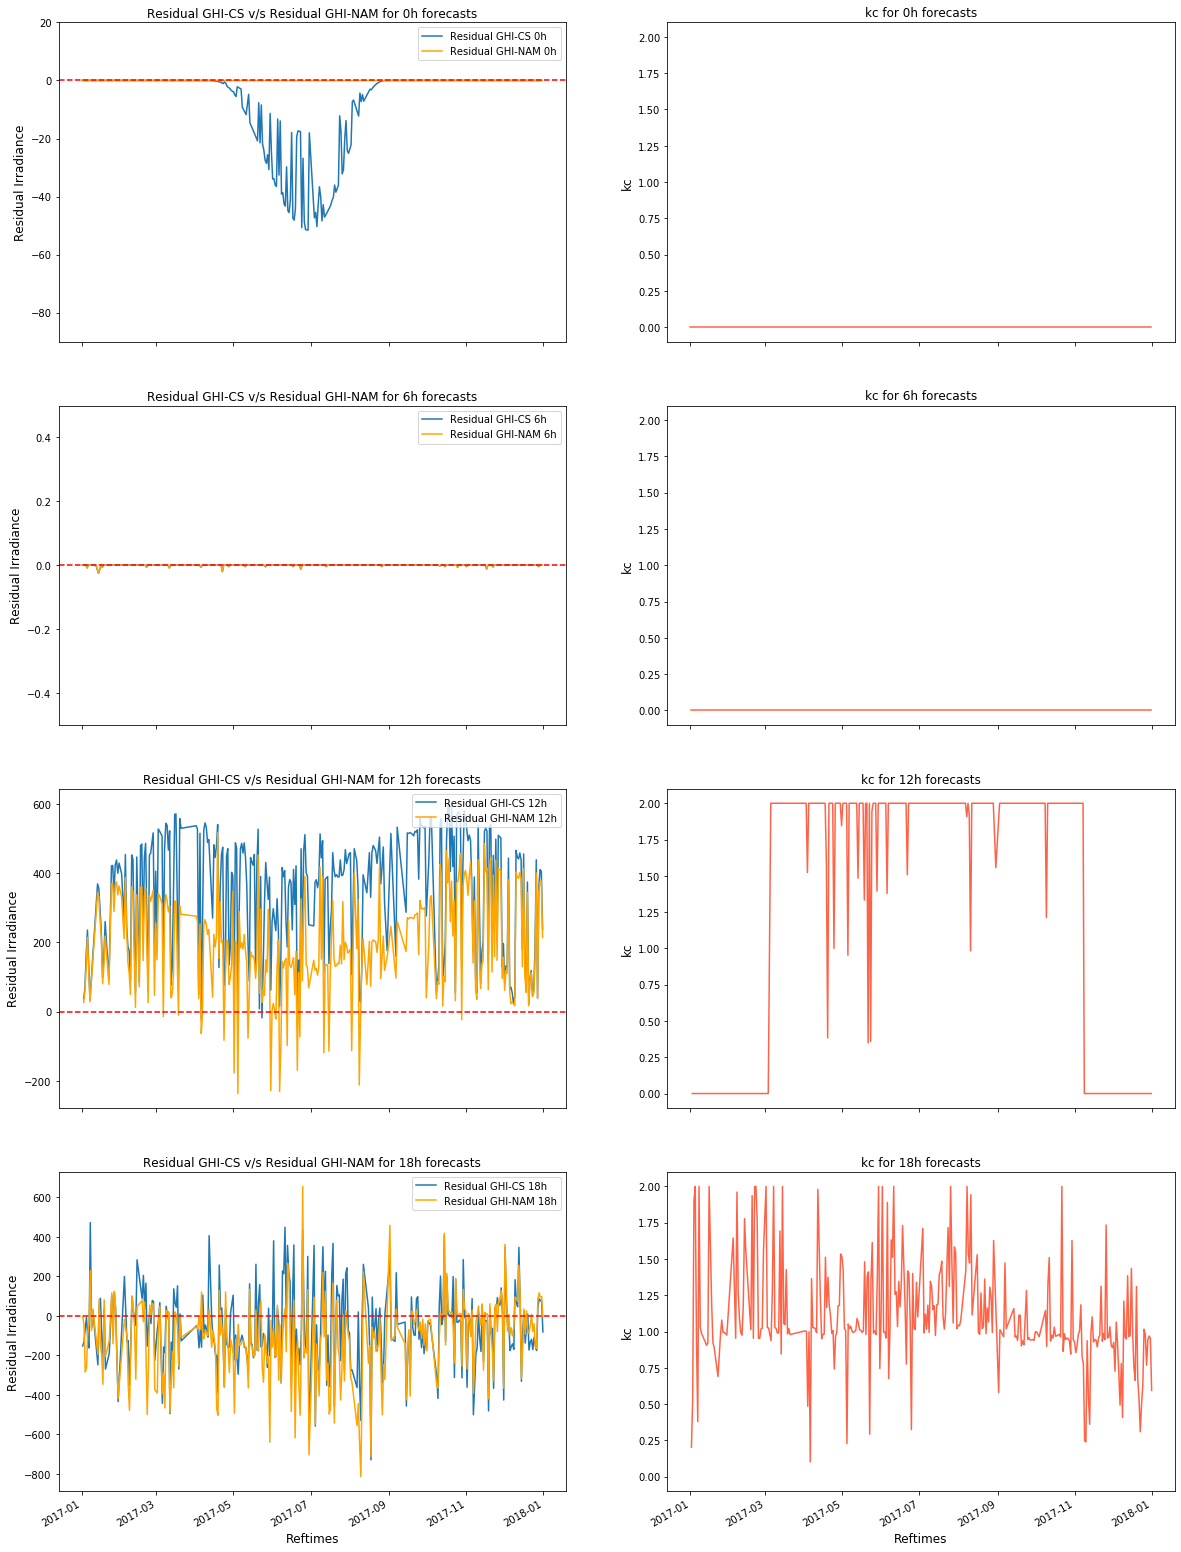
\includegraphics[width=\textwidth]{chapter4/fig_ghi_comparison_cs.png}
    	\caption[Comparing GHI from Clearsky-Scaling ($GHI_{CS}$) and GHI from NAM Forecast Model ($GHI_{NAM}$) for 00h, 06h, 12h, 18h forecasts in 2017]{Comparing GHI from Clearsky-Scaling ($GHI_{CS}$) and GHI from NAM Forecast Model ($GHI_{NAM}$) for 00h, 06h, 12h, 18h forecasts: Residuals of $GHI_{CS}$ and $GHI_{NAM}$ with respect to Array B irradiance observations (left); Clear-sky index ($K_c$) estimations for individual forecasts in 2017 (right).}
    	\label{fig:fig_ghi_comparison_cs}
    \end{center}
\end{figure}

\par In order to assess the $GHI$ values from both NAM model and Clear-Sky Scaling model, residuals between the irradiance observations from solar array B and both $GHI\textsubscript{NAM}$ and $GHI\textsubscript{CS}$ were estimated for the year 2017. Among these, the residuals corresponding to the 00h, 06h, 12h and 18h UTC forecasts were separated, and were plotted in Fig.~\ref{fig:fig_ghi_comparison_cs} (left). The clear-sky index was evaluated for each of the forecasts, and corresponding plots were drawn in Fig.~\ref{fig:fig_ghi_comparison_cs} (right). It was observed that the clear-sky index was constantly zero for the 00h and 06h forecasts throughout the year. This can be attributed to the fact that these forecasts correspond to the time of darkness, resulting in no solar radiation being captured in the solar arrays. Additionally, it can be seen that the residuals for $GHI\textsubscript{NAM}$ are consistently better than the $GHI\textsubscript{CS}$ values for the 12h forecasts, while for the 18h forecasts, they are inconclusive. Thus, the 12h and 18h forecasts were further analyzed with respect to the clear-sky index values.

\begin{table}[h]
\begin{center}
    \caption{MAE of $GHI_{CS}$ and $GHI_{NAM}$ with Array B irradiance for 12h and 18h forecasts.}
    \label{Tab:mean_absolute_residual}
    \begin{tabular}{ c c c c }
    	\toprule
    	\textbf{\parbox{2cm}{\centering Forecast Hour}} & \boldmath\textbf{$K_c$} & \textbf{\parbox{4.5cm}{\centering Mean Absolute Error of \boldmath$GHI_{CS}$}} & \textbf{\parbox{4.5cm}{\centering Mean Absolute Error of \boldmath$GHI_{NAM}$}}\\
    	\midrule
    	\multirow{3}{4em}{$12$} & $< 1.5$ & 271.003 & 219.064 \\ &
    	$> 1.5$ & 383.122 & 204.682 \\
    	\midrule
    	\multirow{3}{4em}{$18$} & $< 1.5$ & 155.63 & 157.38 \\ &
    	$> 1.5$ & 172.869 & 229.998 \\
    	\bottomrule
    \end{tabular}
\end{center}
\end{table}

\par In Table \ref{Tab:mean_absolute_residual}, mean of the absolute values of the residuals (MAE) was computed for the 12h and 18h forecasts, depending on the clear-sky index values estimated for the forecasts. It was observed that for the 12h forecasts, irrespective of $K_c$, $MAE$ corresponding to $GHI_{NAM}$ was lower than that of $GHI_{CS}$, indicating that the GHI predicted by NAM for these forecasts were a better estimation. However, for the 18h forecasts, $MAE$ for forecasts with $K_c < 1.5$ was marginally better for $GHI_{CS}$. Additionally, the $MAE$ for 18h forecasts with $K_c > 1.5$ was significantly better for $GHI_{CS}$, as compared to $GHI_{NAM}$. Thus, it can be concluded that the NAM model tends to overpredict GHI in clear-sky conditions. Thus, in order to correct this bias, for all the 18h forecasts with a $K_c$ value greater than 1.5, $GHI\textsubscript{NAM}$ and $GHI\textsubscript{CS}$ are averaged.

\par From the Clearsky Scaling technique in \textit{pvlib-python}, three irradiance metrics, i.e, GHI, DHI and DNI are retrieved. GHI, which is calculated by scaling total cloud cover, and DNI, which is calculated from the DISC method are highly correlated. Also, DHI, which is empirically calculated from both GHI and DNI, is highly correlated with GHI. Thus, to avoid multicollinearity, the remaining two irradiance metrics, i.e, DHI and DNI are not considered as explanatory variables for the post-processing of irradiance using machine learning models, resulting in the use of only GHI ($GHI_{CS}$) to correct the bias in GHI estimations in NAM model ($GHI_{NAM})$.

\subsubchapter{Blending NAM Forecast Model and Liu-Jordan Model}
The Liu-Jordan Model in \textit{pvlib-python} helps estimate the three irradiance metrics as well. Metrics such as clearness index help in estimating the clearness in the sky and can be determined for a specific day based on collected meteorological data and knowledge of extraterrestrial irradiance. The clearness index for a photovoltaic system can be defined as:
\begin{center}
    $K\textsubscript{t} = \frac{I}{I_0}$
\end{center}
where $I$ is the incoming solar radiation into the earth's atmosphere and $I_0$ is that reaching the ground. For the computation of clearness index, estimation of extraterrestrial radiation for a day of the year, and the estimation of solar zenith angle are necessary. Reda et al. \cite{multimodel_spa} proposed \textit{Solar Position Algorithm}, an implementation of which was used in the determination of the solar zenith angle. The extraterrestrial radiation was determined using an implementation of the algorithm described by Spencer. J in \cite{multimodel_extraterrestrial}. It was formulated such that the negative and non-finite values are truncated to zero, and the maximum value is 2, allowing the over-irradiance events typically seen in sub-hourly data.

\begin{figure}[htbp]
    \begin{center}
    	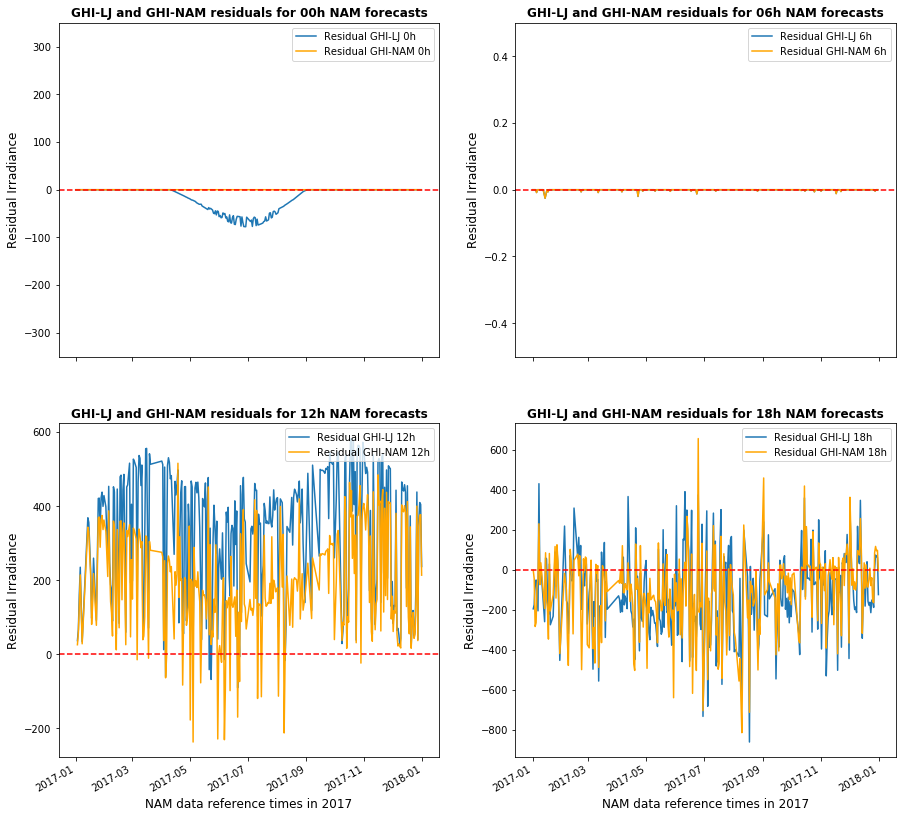
\includegraphics[width=\textwidth]{chapter4/fig_ghi_comparison_lj.png}
    	\caption[Comparing GHI from Liu Jordan Model ($GHI_{LJ}$) and GHI from NAM Forecast Model ($GHI_{NAM}$) for 00h, 06h, 12h, 18h forecasts in 2017]{Comparing GHI from Liu Jordan Model ($GHI_{LJ}$) and GHI from NAM Forecast Model ($GHI_{NAM}$) for 00h, 06h, 12h, 18h forecasts: Residuals of $GHI_{CS}$ and $GHI_{NAM}$ with respect to Array B irradiance observations (left); Clearness index ($K_t$) estimations for individual forecasts in 2017 (right).}
    	\label{fig:fig_ghi_comparison_lj}
    \end{center}
\end{figure}

\par In order to analyze the $GHI$ values from both NAM model and Liu Jordan model, residuals between the irradiance observations from solar array B and both $GHI\textsubscript{NAM}$ and $GHI\textsubscript{LJ}$ were estimated for the year 2017. Among these, the residuals corresponding to the 00h, 06h, 12h and 18h UTC forecasts were separated, and were plotted in Fig.~\ref{fig:fig_ghi_comparison_lj} (left). Clearness index is extremely important in the parameterization of Liu-Jordan model. Thus, it was evaluated for each of the forecasts, and corresponding plots were drawn in Fig.~\ref{fig:fig_ghi_comparison_lj} (right). It was observed that the clearness index too, like clear-sky index in Fig.~\ref{fig:fig_ghi_comparison_lj} was constantly zero for the 06h forecasts throughout the year. This can be attributed to the fact that these forecasts correspond to the time of darkness. However, unlike the clear-sky index metric, which is constantly zero for the 00h forecasts as well, it was observed that the clearness index resulted in a significant non-zero plot for few of the 00h forecasts, indicating that GHI was wrongly estimated for these forecasts, which the clearness metric couldn't ascertain.

\par In the Liu Jordan model, DNI is estimated from transmittance, DHI based on transmittance and solar zenith angle, and GHI is empirically formulated from DHI and DNI. GHI estimated by the Liu Jordan model is blended into the dataset by averaging the GHI estimates for the 18h NAM forecasts, for which $K_t > 0.7$. Furthermore, Liu Jordan model has been shown to be effective in predicting diffuse irradiance on inclined surfaces. This was also verified as the DHI estimated by this model was observed to have a higher correlation with the ground-based solar irradiance observations. Additionally, it was also observed that the GHI observations through this formulation for the year 2017 are highly correlated with DNI. Thus, to avoid multicollinearity amongst the estimators, only DHI estimated by Liu Jordan model was included along with the estimators from the NAM model for the post-processing of solar irradiance using machine learning models.

\subsubchapter{Predictive Modeling Using Clear-Sky Index}

\subchapter{Results and Discussion}
\par In \cite{thesis_zach}, Jones et al used a 24-hour \textit{persistence model} to set a baseline for the more sophisticated machine learning models. In general, persistence models are based on the assumption that conditions remain unchanged between the current time and a future time. The 24-hour persistence models would measure the solar irradiance at a particular time $t$ based on the irradiance value measured at $t-24$. Making use of such a trivial model as a baseline helps in understanding and preparing the data better, by providing a reference for improving the model. Similar 24-hour \textit{persistence models} were used as a baseline in this work as well.

\par Several machine learning algorithms such as least-squares linear regression (LSLR), k-Nearest Neighbors (KNN), Support Vector Regression (SVR), Decision Trees (DT), Random Forests (RF) and Extreme Gradient Boosted Trees (XGBT) were used for the purpose of forecasting. Weather parameter inputs from the NAM data were used as inputs to the machine learning models, and the irradiance observations from the solar arrays A, B and E were used as the target variables. Prediction of target irradiance was done for a forecast horizon of 24 hours, i.e, solar irradiance on each of the arrays was predicted 24 hours into the future, at a one hour temporal resolution. Models were trained on data collected during 2017, and evaluated against data collected during 2018. The performance of the machine learning models were evaluated based on the metrics such as \textit{mean absolute error (MAE)} and $R^2$.  

\par Separate machine learning models were trained for each of the target hour offsets between 1 and 24, and their results were analyzed in two schemes: mean of the evaluations for each forecast hour in the forecast horizon ($Overall$); mean of the evaluations for sets of six forecast hours in the forecast horizon, i.e, $1 - 6$, $7 - 12$, $13 - 18$ and $19 - 24$. Such an analysis helped in realizing the performance of the models specifically for different periods in the day. 

\par In this work, an input selection scheme as described in 3.2 was incorporated towards selecting features for the machine learning models. As a part of this scheme, the key differences between Jones' dataset and the one used in this work, towards training with the machine learning models are as follows: Jones et al hadn't considered the \textit{total cloud cover} parameter in the NAM weather dataset; from among the other surface weather variables used, only air temperature, height at planetary boundary layer and downward shortwave radiation flux were considered; instead of the 36 feature projections for each of the weather variables, select feature projections depending on the target hour offset were chosen; design of the temporal features was different. Based on these differences, the two NAM datasets were used as input to different machine learning models.


\begin{table}[h]
\begin{center}
    \caption{Sample Table 1}
    \begin{tabular}{ c c c c c c c c c}
    	\toprule
    	\textbf{Metric} & \textbf{Horizon} & \textbf{PER} & \textbf{LSLR} & \textbf{SVR} & \textbf{KNN} & \textbf{DT} & \textbf{RF} & \textbf{XGBT}\\
    	\midrule
    	\multirow{3}{4em}{$MAE$} & $1 - 6$ & \_\_ & \_\_ & \_\_ & \_\_ & \_\_ & \_\_ & \_\_\\ &
    	$7 - 12$ & \_\_ & \_\_ & \_\_ & \_\_ & \_\_ & \_\_ & \_\_\\ &
    	$13 - 18$ & \_\_ & \_\_ & \_\_ & \_\_ & \_\_ & \_\_ & \_\_\\ &
    	$19 - 24$ & \_\_ & \_\_ & \_\_ & \_\_ & \_\_ & \_\_ & \_\_\\ &
    	$Overall$ & \_\_ & \_\_ & \_\_ & \_\_ & \_\_ & \_\_ & \_\_\\
    	\midrule
    	\multirow{3}{4em}{$R^2$} & $1 - 6$ & \_\_ & \_\_ & \_\_ & \_\_ & \_\_ & \_\_ & \_\_ \\ &
    	$7 - 12$ & \_\_ & \_\_ & \_\_ & \_\_ & \_\_ & \_\_ & \_\_\\ &
    	$13 - 18$ & \_\_ & \_\_ & \_\_ & \_\_ & \_\_ & \_\_ & \_\_\\ &
    	$19 - 24$ & \_\_ & \_\_ & \_\_ & \_\_ & \_\_ & \_\_ & \_\_\\ &
    	$Overall$ & \_\_ & \_\_ & \_\_ & \_\_ & \_\_ & \_\_ & \_\_\\
    	\bottomrule
    \end{tabular}
\end{center}
\end{table}

\newpage